%% Consolidated float file. Order follows first reference in text:
%% background (market/CDS validation) -> descriptive stats -> results
%% (level DiD, overlay ES, extended ES, triple diff, TD rates, posted rates,
%% brokered, insured wholesale, brokered ES, reciprocal ES, financial,
%% anticipation) -> robustness (predictors, SVB exposure).
%% Notes describe what is done, not what is found.

%% Institutional background

\clearpage
\begin{figure}
    \centering
    \adddescription{
    \small
Event-study estimates for large publicly traded bank holding companies around their 2020Q1 CECL adoption, interacting event-time dummies with each holding company's CECL Day-One adjustment scaled by equity. Panel A uses market capitalization normalized to its first sample month; Panel B uses five-year CDS spreads (basis points) for the 103 holding companies with active contracts and a complete $\pm 9$-month window. The horizontal axis measures months relative to CECL adoption, with month $-1$ omitted as the reference period. Coefficients come from bank and calendar-month fixed-effects regressions with log assets as a control and bank-clustered standard errors. Shaded bands are pointwise 90\% confidence intervals.
    }
    Panel A: Normalized market cap\\
    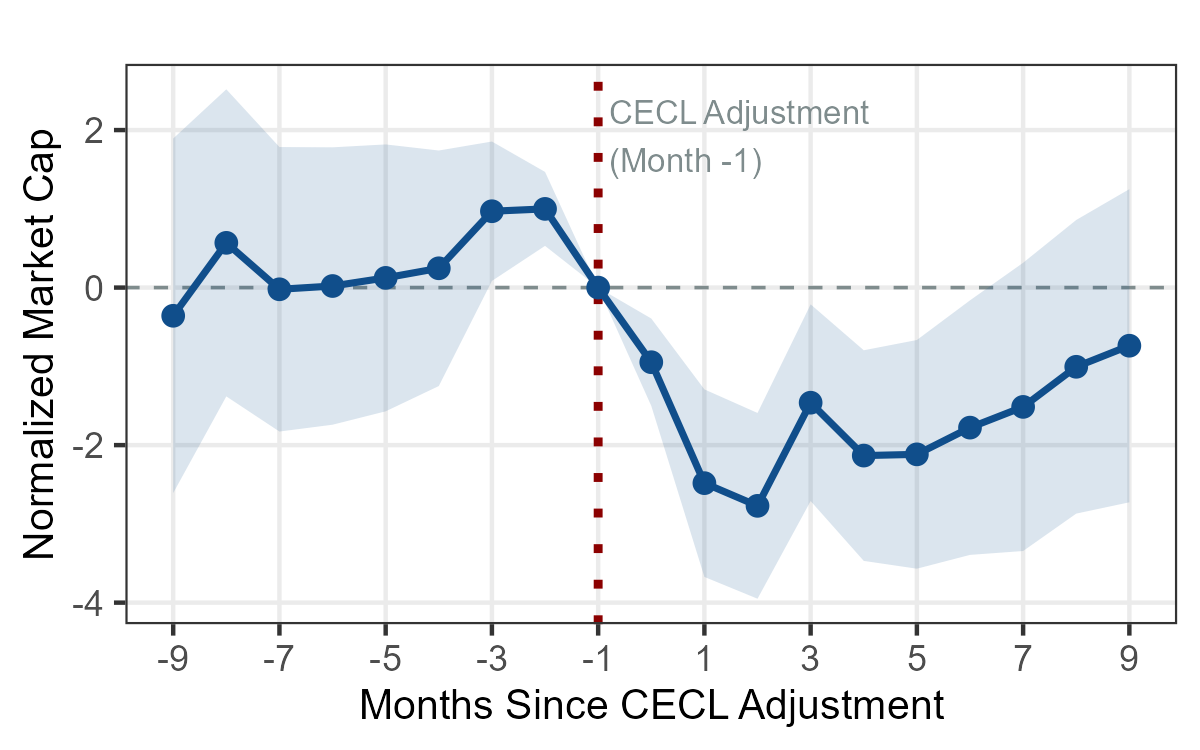
\includegraphics[width=0.75\textwidth]{figures/mkt_cap_large_banks_20260403.png}
    \vspace{0.5cm}\\
    Panel B: CDS spread\\
    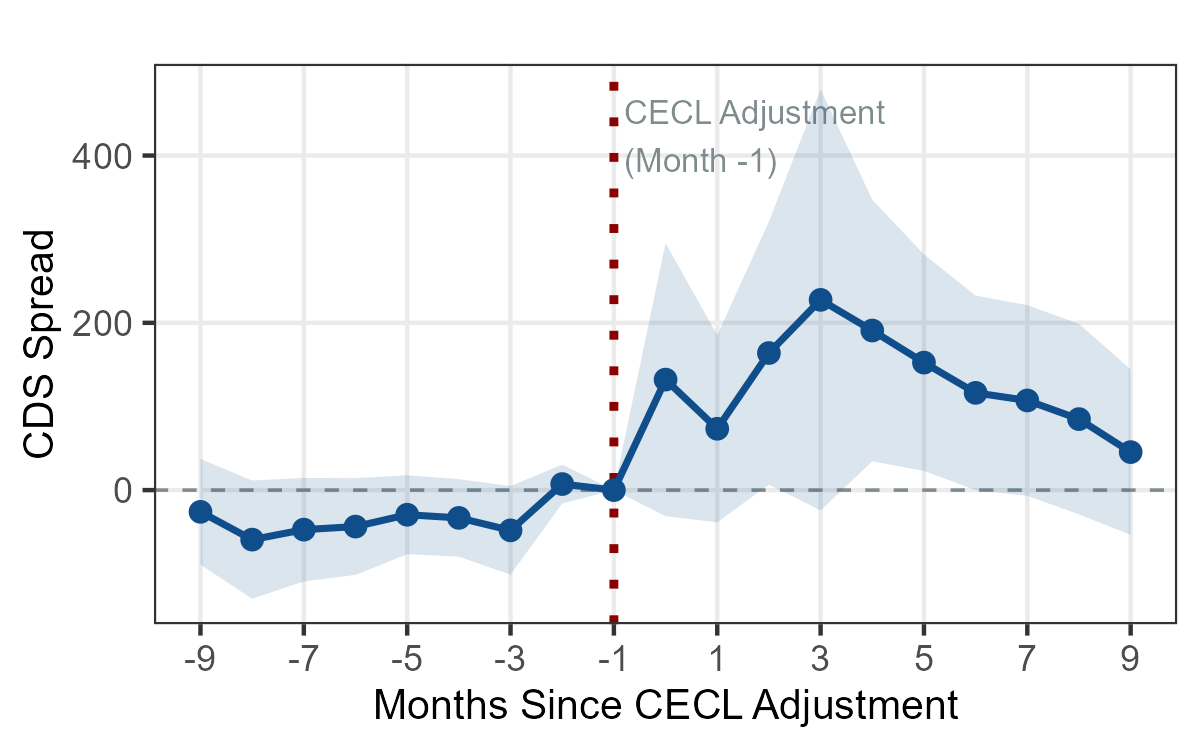
\includegraphics[width=0.75\textwidth]{figures/cds_spread_large_banks_20260403.png}
    \caption{Market validation: equity and CDS responses at large-bank CECL adoption}
    \label{fig:es_large_banks_market_cds}
\end{figure}

%% Descriptive statistics

\clearpage
\begin{figure}
    \centering
    \adddescription{
    \small
This figure plots the cross-sectional distribution of the CECL Day-One retained-earnings adjustment scaled by pre-adoption equity (percentage points) for community banks at the adoption quarter. The vertical dashed line marks the high-CECL threshold of 2.5 percent of equity (approximately the 95th percentile).
    }
    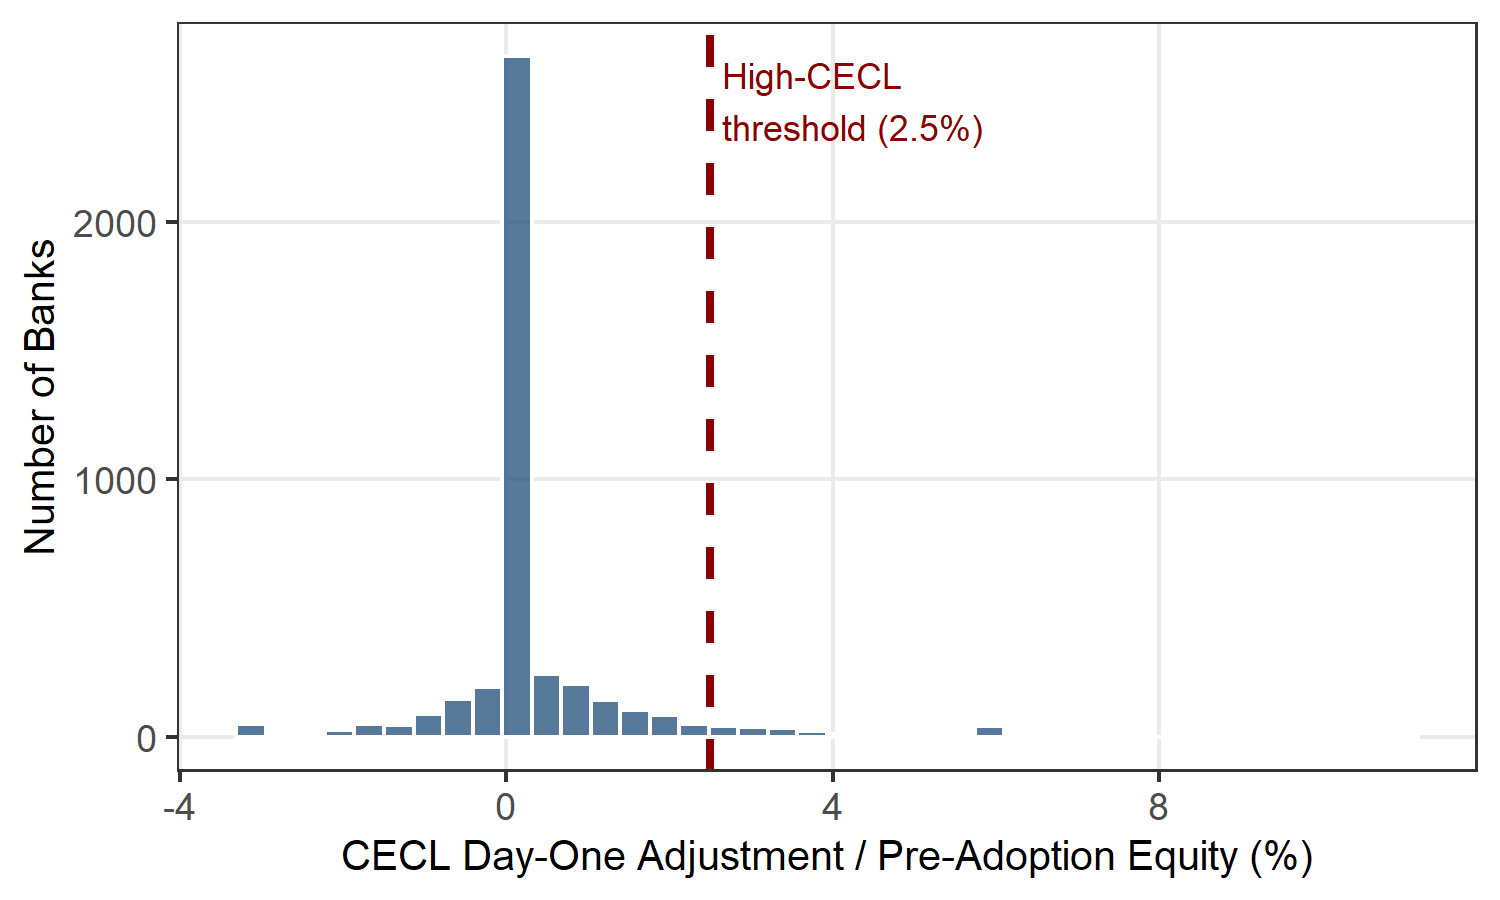
\includegraphics[width=0.75\textwidth]{figures/fig01_cecl_dist_20260612.png}
    \caption{Distribution of CECL adjustment relative to equity}
    \label{fig:cecl_equity_distribution}
\end{figure}

\clearpage
\begin{table}[]
    \centering
    \adddescription{
\small
Summary statistics at each bank's CECL adoption quarter. Columns present the full sample, banks with a high CECL Day-One adjustment (at or above 2.5 percent of equity), the remaining low-CECL banks, and the high-minus-low mean difference with two-sample $t$-test significance. Ratio variables are in percentage points, winsorized within quarter at the 1st and 99th percentiles. *, **, *** denote significance at 10\%, 5\%, 1\%.
    }
    \vspace{0.25cm}
    \resizebox{0.8\textwidth}{!}{\input{tables/tab01_sumstats_20260612}}
    \caption{Summary statistics at CECL adoption}
    \label{tab:descriptive_sumstats_cecl}
\end{table}

%% Main results

\clearpage
\begin{table}[]
    \centering
    \adddescription{
\small
Difference-in-differences estimates. Dependent variables: uninsured time deposits/assets (cols 1--2) and insured time deposits/assets (cols 3--4), in percentage points. Odd columns interact Post with continuous CECL Day-One adjustment relative to equity; even columns use the High-CECL indicator. Bank and calendar-quarter FE; lagged log assets, equity-to-assets, and interest expense/assets. Bank-clustered standard errors. *, **, *** denote 10\%, 5\%, 1\%.
    }
    \vspace{0.25cm}
    \resizebox{0.8\textwidth}{!}{\input{tables/tbl_did_time_deposits_20260612}}
    \caption{Difference-in-differences: time deposits and CECL exposure}
    \label{tab:small_bank_did_time_deposits}
\end{table}

\clearpage
\begin{figure}
    \centering
    \adddescription{
    \small
Event-study estimates for uninsured and insured time deposits/assets, overlaid in a single panel, under the High-CECL indicator interaction. Horizontal axis: quarters relative to each bank's CECL adoption, $k=-1$ omitted. Bank and calendar-quarter FE; lagged controls; bank-clustered standard errors. Shaded bands are pointwise 90\% CIs.
    }
    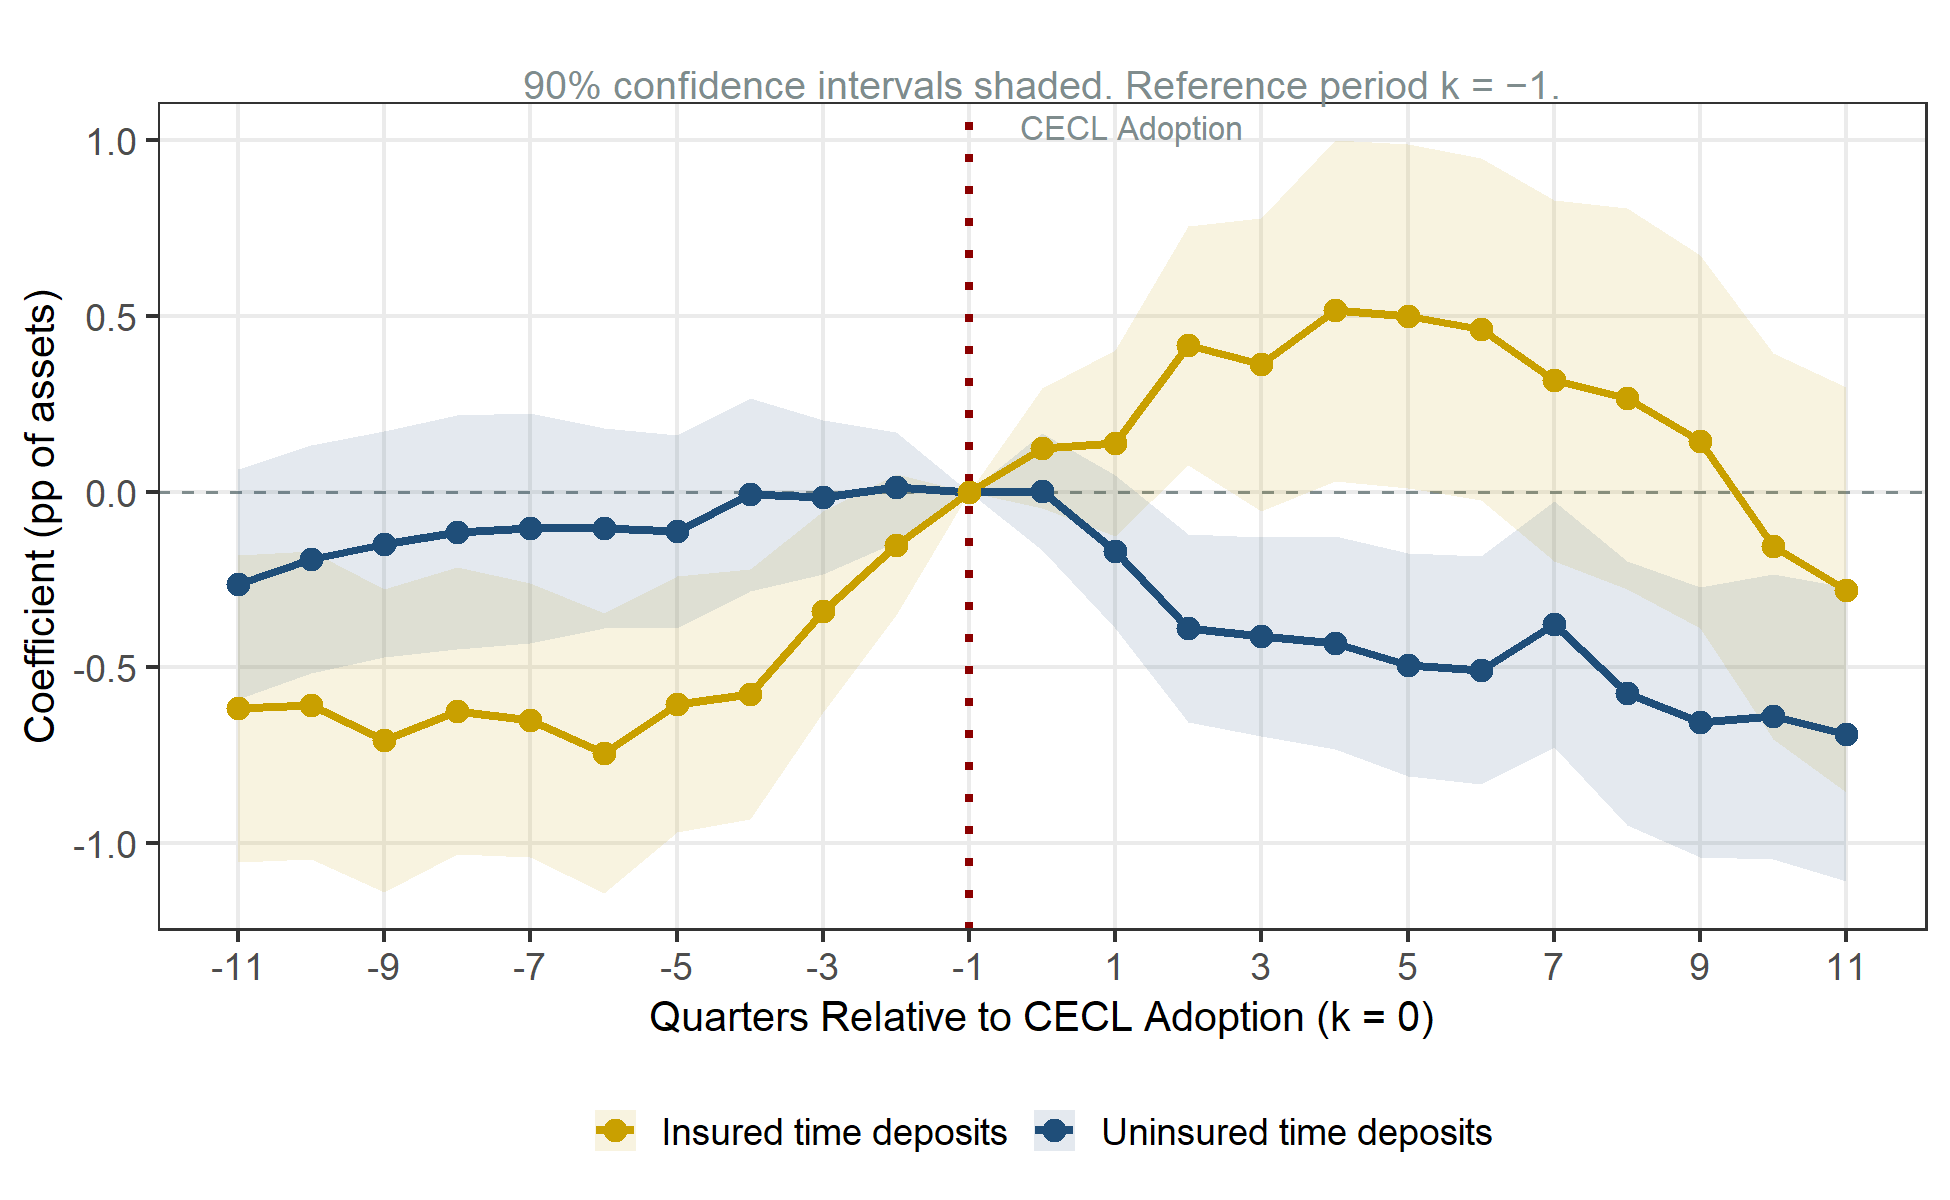
\includegraphics[width=0.85\textwidth]{figures/fig_overlay_composition_20260806.png}
    \caption{Uninsured vs.\ insured time deposits around CECL adoption}
    \label{fig:overlay_composition}
\end{figure}

\clearpage
\begin{figure}
    \centering
    \adddescription{
    \small
Extended event studies from 2018Q1 under the High-CECL indicator. The $k=-20$ coefficient pools all event times at or below $-20$ and the $k=+11$ coefficient pools all event times at or above $+11$, so that edge event times reached only by the small off-cycle cohorts are not estimated from a handful of banks. Panel A: uninsured time deposits/assets. Panel B: insured time deposits/assets. The shaded vertical band marks the COVID-19 quarters (2020Q1--Q2) for the 2023Q1 cohort. Bank and calendar-quarter FE; lagged controls; bank-clustered SEs; shaded bands are 90\% CIs.
    }
    \begin{minipage}[t]{0.49\textwidth}
        \centering
        {\small Panel A: Uninsured time deposits/assets}\\[-0.25em]
        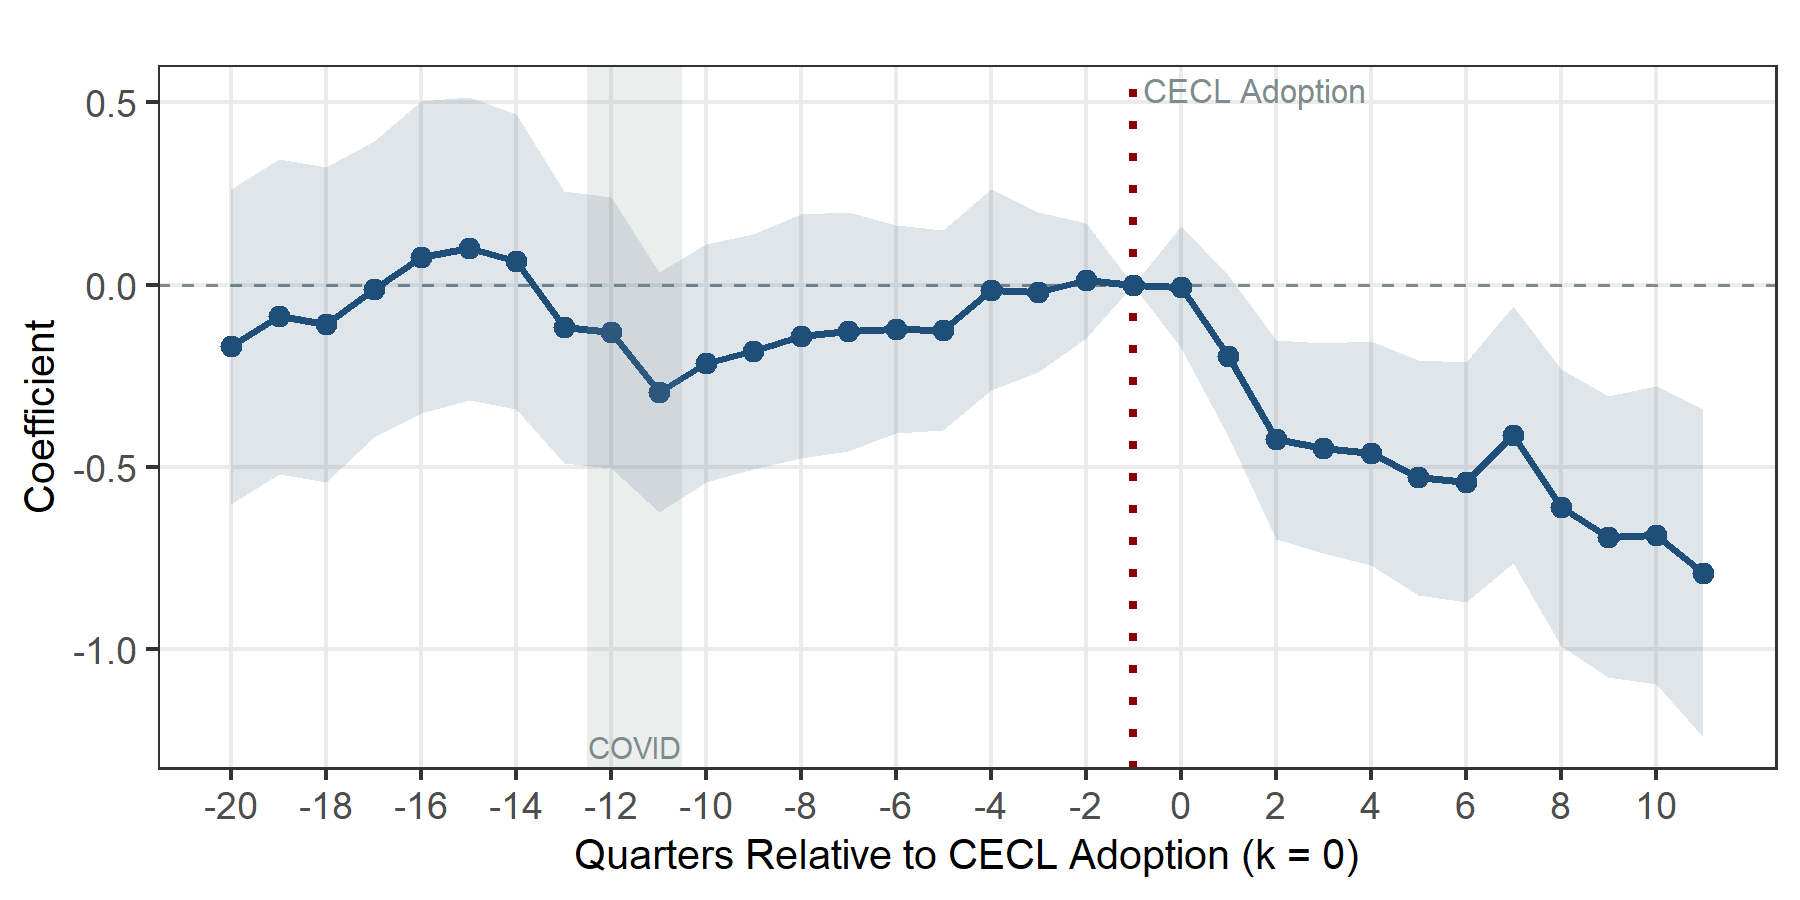
\includegraphics[width=\linewidth]{figures/fig_es_long_unins_balanced_20260806.png}
    \end{minipage}\hfill
    \begin{minipage}[t]{0.49\textwidth}
        \centering
        {\small Panel B: Insured time deposits/assets}\\[-0.25em]
        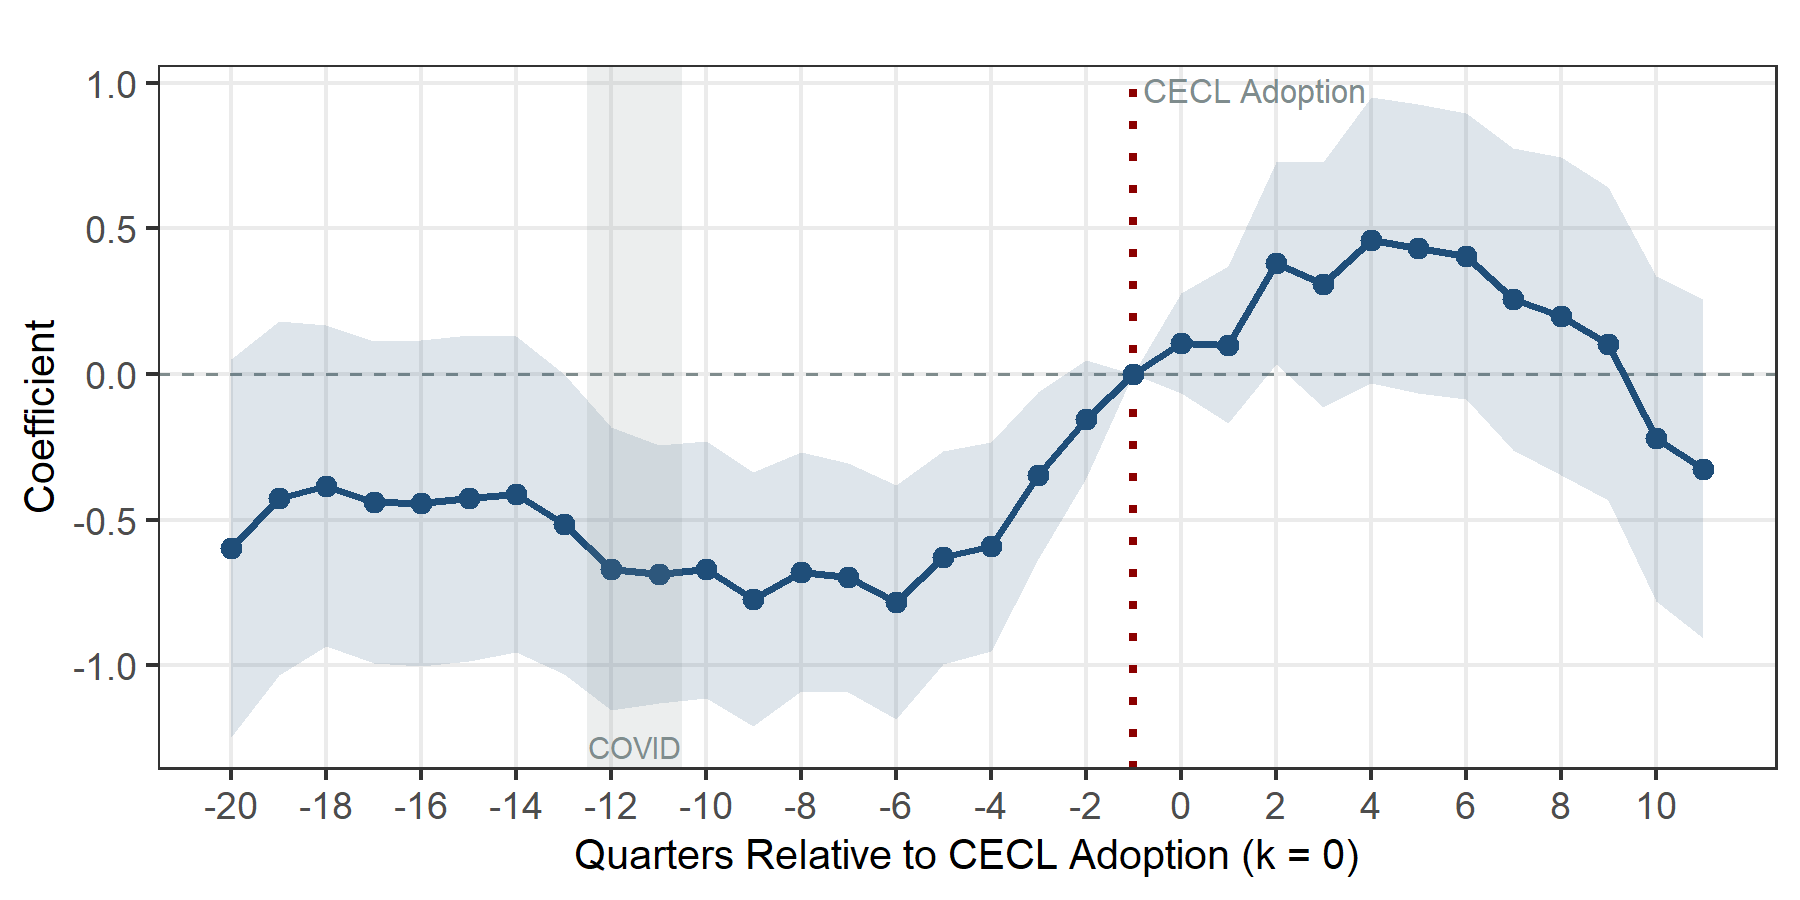
\includegraphics[width=\linewidth]{figures/fig_es_long_ins_balanced_20260806.png}
    \end{minipage}
    \caption{Extended event studies, 2018Q1 onward}
    \label{fig:es_long_balanced}
\end{figure}

\clearpage
\begin{table}[]
    \centering
    \adddescription{
\small
Triple-difference estimates. Stacked panel: each bank-quarter contributes two rows (uninsured and insured time deposits/assets) with an uninsured indicator. Column (1) uses continuous CECL adjustment relative to equity; column (2) uses the High-CECL indicator. Bank $\times$ quarter fixed effects absorb all bank-specific time-varying shocks; identification comes from the within-bank, within-quarter uninsured-vs-insured differential. Bank-clustered standard errors. *, **, *** denote 10\%, 5\%, 1\%.
    }
    \vspace{0.25cm}
    \resizebox{0.8\textwidth}{!}{\input{tables/tbl_triple_diff_time_deposits_20260612}}
    \caption{Triple difference: time deposits, CECL, and uninsured status}
    \label{tab:small_bank_triple_diff_time_deposits}
\end{table}

\clearpage
\begin{table}[]
    \centering
    \adddescription{
\small
Difference-in-differences estimates interacted with the pre-adoption capital buffer. The moderator is each bank's equity-to-assets ratio frozen at 2022Q4 and winsorized at the bank-level 1st and 99th percentiles. Dependent variables: uninsured time deposits/assets (cols 1--3) and the within-bank gap between uninsured and insured time deposits/assets (cols 4--6), which is the outcome underlying the bank $\times$ quarter triple difference. Columns (1), (3), (4), and (6) include lagged log assets, equity-to-assets, and interest expense/assets; columns (2) and (5) drop the lagged equity control. Columns (3) and (6) use the High-CECL indicator in place of the continuous adjustment. Bank and calendar-quarter FE; bank-clustered standard errors. *, **, *** denote 10\%, 5\%, 1\%.
    }
    \vspace{0.25cm}
    \resizebox{\textwidth}{!}{
\begingroup
\centering
\begin{tabular}{lcccccc}
   \tabularnewline \midrule \midrule
   Dependent Variables: & \multicolumn{3}{c}{Unins. Time Dep./Assets (\%)} & \multicolumn{3}{c}{Unins. $-$ Ins. Time Deps/Assets (\%)}\\
   Model:                           & (1)             & (2)             & (3)             & (4)             & (5)             & (6)\\  
   \midrule
   \emph{Variables}\\
   Post x CECL Adj x Equity 2022Q4  & 0.0275$^{**}$   & 0.0285$^{**}$   &                 & 0.0665$^{***}$  & 0.0659$^{***}$  &   \\   
                                    & (0.0140)        & (0.0140)        &                 & (0.0194)        & (0.0195)        &   \\   
   Post x High CECL x Equity 2022Q4 &                 &                 & 0.0898          &                 &                 & 0.3074$^{***}$\\   
                                    &                 &                 & (0.0673)        &                 &                 & (0.1147)\\   
   Post x CECL Adj                  & -0.3476$^{**}$  & -0.3595$^{**}$  &                 & -0.8009$^{***}$ & -0.7939$^{***}$ &   \\   
                                    & (0.1402)        & (0.1397)        &                 & (0.2101)        & (0.2103)        &   \\   
   Post x High CECL                 &                 &                 & -1.294$^{*}$    &                 &                 & -4.117$^{***}$\\   
                                    &                 &                 & (0.6649)        &                 &                 & (1.264)\\   
   Post                             & 0.2766$^{**}$   & 0.2727$^{**}$   & 0.2662$^{**}$   & 0.0442          & 0.0466          & 0.0509\\   
                                    & (0.1218)        & (0.1216)        & (0.1220)        & (0.1911)        & (0.1928)        & (0.1924)\\   
   log(Assets), $t{-}1$             & -0.3624         & -0.1767         & -0.3781         & -0.4474         & -0.5581$^{*}$   & -0.4640\\   
                                    & (0.2364)        & (0.2325)        & (0.2353)        & (0.3359)        & (0.3238)        & (0.3336)\\   
   Equity/Assets (\%), $t{-}1$      & -0.0555$^{***}$ &                 & -0.0559$^{***}$ & 0.0331$^{*}$    &                 & 0.0324$^{*}$\\   
                                    & (0.0112)        &                 & (0.0113)        & (0.0197)        &                 & (0.0197)\\   
   Int. Exp/Assets (\%), $t{-}1$    & 4.934$^{***}$   & 4.937$^{***}$   & 4.932$^{***}$   & -1.160$^{**}$   & -1.162$^{**}$   & -1.148$^{**}$\\   
                                    & (0.3166)        & (0.3194)        & (0.3172)        & (0.4928)        & (0.4933)        & (0.4935)\\   
   Post x Equity 2022Q4             & -0.0196$^{***}$ & -0.0190$^{***}$ & -0.0184$^{***}$ & 0.0133          & 0.0129          & 0.0149\\   
                                    & (0.0070)        & (0.0070)        & (0.0071)        & (0.0111)        & (0.0112)        & (0.0112)\\   
   \midrule
   \emph{Fixed-effects}\\
   Bank                             & Yes             & Yes             & Yes             & Yes             & Yes             & Yes\\  
   Quarter                          & Yes             & Yes             & Yes             & Yes             & Yes             & Yes\\  
   \midrule
   \emph{Fit statistics}\\
   Observations                     & 97,064          & 97,064          & 97,064          & 97,064          & 97,064          & 97,064\\  
   Adjusted R$^2$                   & 0.82141         & 0.82088         & 0.82136         & 0.75880         & 0.75868         & 0.75889\\  
   \midrule \midrule
   \multicolumn{7}{l}{\emph{Clustered (Bank) standard-errors in parentheses}}\\
   \multicolumn{7}{l}{\emph{Signif. Codes: ***: 0.01, **: 0.05, *: 0.1}}\\
\end{tabular}
\par\endgroup


}
    \caption{Disclosure response and the pre-adoption capital buffer}
    \label{tab:capital_het}
\end{table}

\clearpage
\begin{table}[]
    \centering
    \adddescription{
\small
Difference-in-differences estimates for implied time-deposit rates. Dependent variables: implied annualized rate on uninsured time deposits (interest expense on time deposits above \$250{,}000 over average balances in that category; cols 1--2), implied rate on insured time deposits (interest on time deposits at or below \$250{,}000 over the matching balances; cols 3--4), and the within-bank spread between the two (cols 5--6), in annualized percent. Odd columns use continuous CECL adjustment; even use High-CECL. Bank and calendar-quarter FE; lagged log assets and equity-to-assets. Rates winsorized within quarter at the 1st and 99th percentiles; bank-quarters with average category balances below \$250{,}000 excluded. Bank-clustered standard errors. *, **, *** denote 10\%, 5\%, 1\%.
    }
    \vspace{0.25cm}
    \resizebox{0.9\textwidth}{!}{
\begingroup
\centering
\begin{tabular}{lcccccc}
   \tabularnewline \midrule \midrule
   Dependent Variables: & \multicolumn{2}{c}{Unins. TD Rate (\%)} & \multicolumn{2}{c}{Ins. TD Rate (\%)} & \multicolumn{2}{c}{TD Rate Spread (\%)}\\
   Model:                       & (1)            & (2)            & (3)            & (4)            & (5)             & (6)\\  
   \midrule
   \emph{Variables}\\
   Post x CECL Adj              & -0.0080        &                & 0.0023         &                & -0.0076         &   \\   
                                & (0.0094)       &                & (0.0076)       &                & (0.0099)        &   \\   
   Post x High CECL             &                & -0.0819        &                & 0.0239         &                 & -0.1103$^{*}$\\   
                                &                & (0.0518)       &                & (0.0382)       &                 & (0.0574)\\   
   Post                         & 0.0195         & 0.0211         & 0.0085         & 0.0080         & 0.0023          & 0.0054\\   
                                & (0.0458)       & (0.0458)       & (0.0342)       & (0.0342)       & (0.0515)        & (0.0515)\\   
   log(Assets), $t{-}1$         & 0.3224$^{***}$ & 0.3236$^{***}$ & 0.6387$^{***}$ & 0.6384$^{***}$ & -0.2935$^{***}$ & -0.2907$^{***}$\\   
                                & (0.0456)       & (0.0457)       & (0.0396)       & (0.0396)       & (0.0460)        & (0.0459)\\   
   Equity/Assets (\%), $t{-}1$  & 0.0064$^{**}$  & 0.0064$^{*}$   & 0.0047$^{*}$   & 0.0047$^{*}$   & -0.0018         & -0.0018\\   
                                & (0.0033)       & (0.0033)       & (0.0027)       & (0.0027)       & (0.0036)        & (0.0036)\\   
   \midrule
   \emph{Fixed-effects}\\
   Bank                         & Yes            & Yes            & Yes            & Yes            & Yes             & Yes\\  
   Quarter                      & Yes            & Yes            & Yes            & Yes            & Yes             & Yes\\  
   \midrule
   \emph{Fit statistics}\\
   Observations                 & 93,489         & 93,489         & 95,507         & 95,507         & 93,164          & 93,164\\  
   Adjusted R$^2$               & 0.79421        & 0.79423        & 0.89444        & 0.89444        & 0.23306         & 0.23320\\  
   \midrule \midrule
   \multicolumn{7}{l}{\emph{Clustered (Bank) standard-errors in parentheses}}\\
   \multicolumn{7}{l}{\emph{Signif. Codes: ***: 0.01, **: 0.05, *: 0.1}}\\
\end{tabular}
\par\endgroup


}
    \caption{Implied rates on uninsured vs.\ insured time deposits}
    \label{tab:td_rates}
\end{table}

\clearpage
\begin{table}[]
    \centering
    \adddescription{
\small
Posted deposit rates around the 2023 stress and the Day-One disclosures. Bank-week panel of posted APYs from RateWatch for banks adopting CECL in 2023Q1, July 2022--April 2024: 12-month CDs at the \$10{,}000 tier (col 1) and \$100{,}000 tier (col 2), and savings accounts at the \$2{,}500 tier (col 3). The stress-window indicator covers March 10--April 30, 2023 (after the SVB failure, before 2023Q1 Call Reports were public); the post-publication indicator covers May 1, 2023 onward. Both are interacted with the High-CECL indicator. Bank and week FE; bank-clustered standard errors. *, **, *** denote 10\%, 5\%, 1\%.
    }
    \vspace{0.25cm}
    \resizebox{0.75\textwidth}{!}{
\begingroup
\centering
\begin{tabular}{lccc}
   \tabularnewline \midrule \midrule
   Dependent Variable: & \multicolumn{3}{c}{Posted APY (\%)}\\
   Model:                       & (1)      & (2)      & (3)\\  
   \midrule
   \emph{Variables}\\
   Post-publication x High CECL & -0.0582  & -0.0680  & 0.0081\\   
                                & (0.0737) & (0.0769) & (0.0312)\\   
   Stress x High CECL           & -0.0263  & -0.0252  & 0.0153\\   
                                & (0.0484) & (0.0540) & (0.0231)\\   
   \midrule
   \emph{Fixed-effects}\\
   Bank                         & Yes      & Yes      & Yes\\  
   Week                         & Yes      & Yes      & Yes\\  
   \midrule
   \emph{Fit statistics}\\
   Observations                 & 238,412  & 258,908  & 236,920\\  
   Adjusted R$^2$               & 0.83359  & 0.80945  & 0.83855\\  
   \midrule \midrule
   \multicolumn{4}{l}{\emph{Clustered (Bank) standard-errors in parentheses}}\\
   \multicolumn{4}{l}{\emph{Signif. Codes: ***: 0.01, **: 0.05, *: 0.1}}\\
\end{tabular}
\par\endgroup


}
    \caption{Posted deposit rates around the 2023 stress and the Day-One disclosures}
    \label{tab:rw_did}
\end{table}

\clearpage
\begin{table}[]
    \centering
    \adddescription{
\small
DiD for wholesale and insurance-structured funding outcomes, each scaled by assets (percentage points): total brokered (cols 1--2), insured brokered (cols 3--4), uninsured brokered maturing within one year (cols 5--6), reciprocal deposits (cols 7--8). Odd columns continuous; even High-CECL. Bank and calendar-quarter FE; lagged controls; bank-clustered SEs. *, **, *** denote 10\%, 5\%, 1\%.
    }
    \vspace{0.25cm}
    \resizebox{\textwidth}{!}{
\begingroup
\centering
\begin{tabular}{lcccccccc}
   \tabularnewline \midrule \midrule
   Dependent Variables: & \multicolumn{2}{c}{Brokered Dep./Assets (\%)} & \multicolumn{2}{c}{Ins. Brokered Dep./Assets (\%)} & \multicolumn{2}{c}{Unins. Brokered Dep./Assets (\%)} & \multicolumn{2}{c}{Reciprocal Dep./Assets (\%)}\\
   Model:                         & (1)           & (2)           & (3)           & (4)           & (5)             & (6)             & (7)            & (8)\\  
   \midrule
   \emph{Variables}\\
   Post x CECL Adj                & 0.0666        &               & 0.0860$^{*}$  &               & -0.0014         &                 & 0.0888$^{*}$   &   \\   
                                  & (0.0477)      &               & (0.0483)      &               & (0.0076)        &                 & (0.0462)       &   \\   
   Post x High CECL               &               & 0.4741$^{*}$  &               & 0.5209$^{**}$ &                 & 0.0009          &                & 0.2899\\   
                                  &               & (0.2551)      &               & (0.2644)      &                 & (0.0411)        &                & (0.2525)\\   
   Post                           & -0.1361       & -0.1392       & -0.1648       & -0.1645       & 0.0191          & 0.0187          & 0.0773         & 0.0894\\   
                                  & (0.1093)      & (0.1092)      & (0.1039)      & (0.1033)      & (0.0246)        & (0.0246)        & (0.0675)       & (0.0673)\\   
   log(Assets), $t{-}1$           & 2.067$^{***}$ & 2.070$^{***}$ & 1.936$^{***}$ & 1.943$^{***}$ & 0.0517          & 0.0512          & 2.589$^{***}$  & 2.604$^{***}$\\   
                                  & (0.3696)      & (0.3691)      & (0.3481)      & (0.3477)      & (0.0315)        & (0.0315)        & (0.3060)       & (0.3072)\\   
   Equity/Assets (\%), $t{-}1$    & 0.0161        & 0.0164        & 0.0304$^{*}$  & 0.0307$^{*}$  & -0.0055$^{***}$ & -0.0055$^{***}$ & 0.0645$^{***}$ & 0.0648$^{***}$\\   
                                  & (0.0192)      & (0.0192)      & (0.0183)      & (0.0182)      & (0.0018)        & (0.0018)        & (0.0114)       & (0.0114)\\   
   Int. Exp/Assets (\%), $t{-}1$  & 7.811$^{***}$ & 7.804$^{***}$ & 7.289$^{***}$ & 7.284$^{***}$ & 0.1795$^{***}$  & 0.1790$^{***}$  & 3.786$^{***}$  & 3.795$^{***}$\\   
                                  & (0.4636)      & (0.4642)      & (0.4559)      & (0.4567)      & (0.0550)        & (0.0551)        & (0.3591)       & (0.3586)\\   
   \midrule
   \emph{Fixed-effects}\\
   Bank                           & Yes           & Yes           & Yes           & Yes           & Yes             & Yes             & Yes            & Yes\\  
   Quarter                        & Yes           & Yes           & Yes           & Yes           & Yes             & Yes             & Yes            & Yes\\  
   \midrule
   \emph{Fit statistics}\\
   Observations                   & 97,064        & 97,064        & 97,064        & 97,064        & 97,064          & 97,064          & 97,056         & 97,056\\  
   Adjusted R$^2$                 & 0.76892       & 0.76897       & 0.75722       & 0.75725       & 0.46456         & 0.46455         & 0.80570        & 0.80562\\  
   \midrule \midrule
   \multicolumn{9}{l}{\emph{Clustered (Bank) standard-errors in parentheses}}\\
   \multicolumn{9}{l}{\emph{Signif. Codes: ***: 0.01, **: 0.05, *: 0.1}}\\
\end{tabular}
\par\endgroup


}
    \caption{Destination of funding: brokered and reciprocal deposits}
    \label{tab:brokered}
\end{table}

\clearpage
\begin{table}[]
    \centering
    \adddescription{
\small
DiD for combined insured wholesale funding. Dependent variables: the sum of insured brokered and reciprocal deposits scaled by assets (percentage points; cols 1--2) and an indicator for holding any reciprocal balance (cols 3--4). Odd columns interact Post with continuous CECL adjustment; even columns use the High-CECL indicator. Bank and calendar-quarter FE; lagged log assets, equity-to-assets, and interest expense/assets. Bank-clustered standard errors. *, **, *** denote 10\%, 5\%, 1\%.
    }
    \vspace{0.25cm}
    \resizebox{0.85\textwidth}{!}{
\begingroup
\centering
\begin{tabular}{lcccc}
   \tabularnewline \midrule \midrule
   Dependent Variables: & \multicolumn{2}{c}{Ins. Brokered + Reciprocal/Assets (\%)} & \multicolumn{2}{c}{Any Reciprocal (0/1)}\\
   Model:                         & (1)            & (2)            & (3)            & (4)\\  
   \midrule
   \emph{Variables}\\
   Post x CECL Adj                & 0.1748$^{**}$  &                & 0.0028         &   \\   
                                  & (0.0723)       &                & (0.0046)       &   \\   
   Post x High CECL               &                & 0.8108$^{**}$  &                & 0.0067\\   
                                  &                & (0.3919)       &                & (0.0227)\\   
   Post                           & -0.0875        & -0.0751        & -0.0050        & -0.0045\\   
                                  & (0.1274)       & (0.1267)       & (0.0115)       & (0.0115)\\   
   log(Assets), $t{-}1$           & 4.525$^{***}$  & 4.548$^{***}$  & 0.1958$^{***}$ & 0.1964$^{***}$\\   
                                  & (0.5419)       & (0.5424)       & (0.0188)       & (0.0189)\\   
   Equity/Assets (\%), $t{-}1$    & 0.0949$^{***}$ & 0.0955$^{***}$ & 0.0015$^{*}$   & 0.0015$^{*}$\\   
                                  & (0.0222)       & (0.0222)       & (0.0009)       & (0.0009)\\   
   Int. Exp/Assets (\%), $t{-}1$  & 11.08$^{***}$  & 11.08$^{***}$  & 0.1597$^{***}$ & 0.1601$^{***}$\\   
                                  & (0.6360)       & (0.6363)       & (0.0296)       & (0.0296)\\   
   \midrule
   \emph{Fixed-effects}\\
   Bank                           & Yes            & Yes            & Yes            & Yes\\  
   Quarter                        & Yes            & Yes            & Yes            & Yes\\  
   \midrule
   \emph{Fit statistics}\\
   Observations                   & 97,056         & 97,056         & 97,056         & 97,056\\  
   Adjusted R$^2$                 & 0.81319        & 0.81314        & 0.79830        & 0.79829\\  
   \midrule \midrule
   \multicolumn{5}{l}{\emph{Clustered (Bank) standard-errors in parentheses}}\\
   \multicolumn{5}{l}{\emph{Signif. Codes: ***: 0.01, **: 0.05, *: 0.1}}\\
\end{tabular}
\par\endgroup


}
    \caption{Combined insured wholesale funding: insured brokered plus reciprocal deposits}
    \label{tab:ins_wholesale}
\end{table}

\clearpage
\begin{figure}
    \centering
    \adddescription{
    \small
Event-study estimates for insured brokered deposits/assets around CECL adoption, under the High-CECL indicator interaction. Horizontal axis: quarters relative to adoption, $k=-1$ omitted. Bank and calendar-quarter FE; lagged controls; bank-clustered SEs; shaded bands are 90\% CIs.
    }
    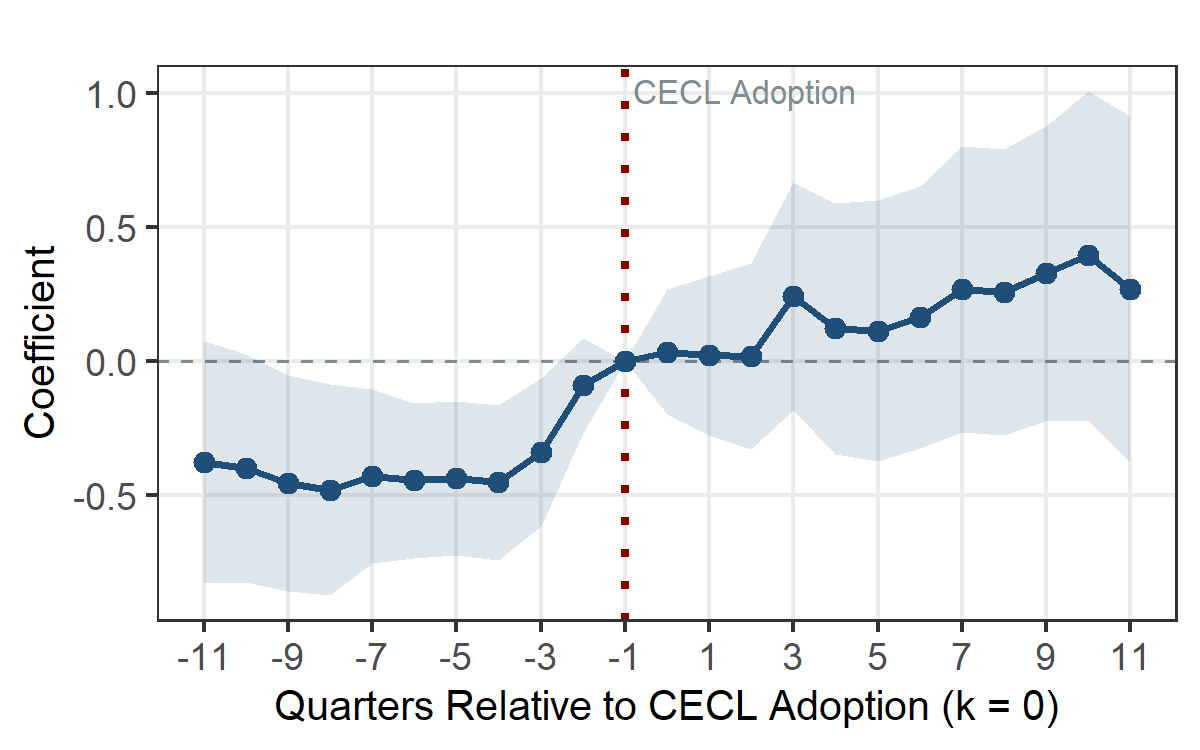
\includegraphics[width=0.7\textwidth]{figures/fig_es_brokered_ins_20260612.png}
    \caption{Event study: insured brokered deposits}
    \label{fig:es_brokered_ins}
\end{figure}

\clearpage
\begin{figure}
    \centering
    \adddescription{
    \small
Event-study estimates for reciprocal deposits/assets around CECL adoption, under the High-CECL indicator interaction. Horizontal axis: quarters relative to adoption, $k=-1$ omitted. Bank and calendar-quarter FE; lagged controls; bank-clustered SEs; shaded bands are 90\% CIs.
    }
    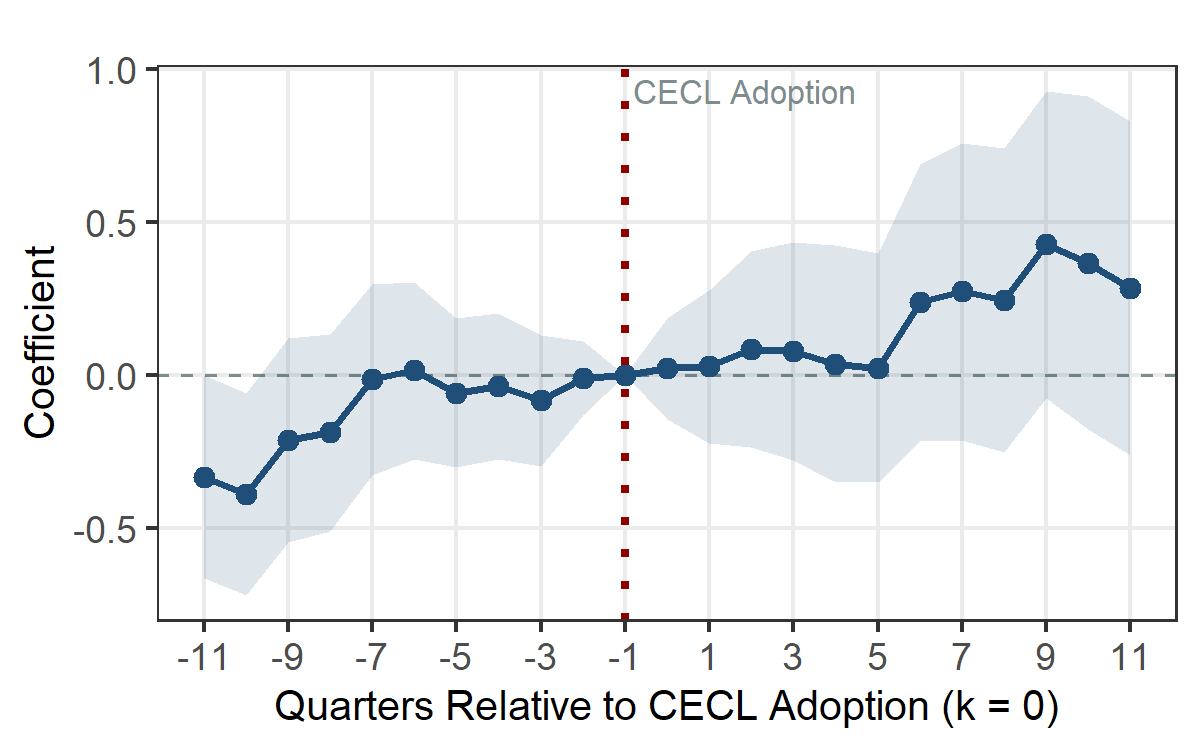
\includegraphics[width=0.7\textwidth]{figures/fig_es_reciprocal_20260612.png}
    \caption{Event study: reciprocal deposits}
    \label{fig:es_reciprocal}
\end{figure}

\clearpage
\begin{table}[]
    \centering
    \adddescription{
\small
Difference-in-differences estimates for financial outcomes. Dependent variables: interest expense/assets (cols 1--2), ROA (cols 3--4), and NIM (cols 5--6), each in quarterly percentage points. Odd columns use continuous CECL adjustment; even use High-CECL. Bank and calendar-quarter FE; lagged log assets and equity-to-assets. Bank-clustered standard errors. *, **, *** denote 10\%, 5\%, 1\%.
    }
    \vspace{0.25cm}
    \resizebox{0.8\textwidth}{!}{\input{tables/tbl_did_financial_outcomes_20260612}}
    \caption{Difference-in-differences: financial outcomes and CECL exposure}
    \label{tab:small_bank_did_financial_outcomes}
\end{table}

\clearpage
\begin{table}[]
    \centering
    \adddescription{
\small
Bank anticipation of the Day-One charge. Columns (1)--(2): cross-sectional regressions of the change in insured brokered deposits/assets over event quarters $-4$ to $-1$ (before any public disclosure) on the future CECL adjustment (col 1 continuous, col 2 High-CECL indicator), with controls measured at event quarter $-4$. Column (3): linear probability model of electing the CECL regulatory capital transition phase-in on the continuous adjustment. Column (4): the pre-adoption brokered change on the election indicator. Heteroskedasticity-robust standard errors. *, **, *** denote 10\%, 5\%, 1\%.
    }
    \vspace{0.25cm}
    \resizebox{0.85\textwidth}{!}{
\begingroup
\centering
\begin{tabular}{lcccc}
   \tabularnewline \midrule \midrule
   Dependent Variables: & \multicolumn{2}{c}{$\Delta$ Ins. Brokered/Assets ($k{=}{-}4$ to $-1$)} & Phase-In Elected & $\Delta$ Ins. Brokered/Assets ($k{=}{-}4$ to $-1$)\\
   Model:                       & (1)            & (2)            & (3)            & (4)\\  
   \midrule
   \emph{Variables}\\
   Constant                     & -3.597$^{***}$ & -3.626$^{***}$ & 0.0493$^{***}$ & -3.459$^{***}$\\   
                                & (0.4318)       & (0.4342)       & (0.0031)       & (0.4272)\\   
   CECL Adj                     & 0.1225$^{***}$ &                & 0.0717$^{***}$ &   \\   
                                & (0.0365)       &                & (0.0054)       &   \\   
   log(Assets), $t{-}1$         & 0.3239$^{***}$ & 0.3266$^{***}$ &                & 0.3138$^{***}$\\   
                                & (0.0341)       & (0.0344)       &                & (0.0339)\\   
   Equity/Assets (\%), $t{-}1$  & 0.0013         & 0.0015         &                & 0.0009\\   
                                & (0.0028)       & (0.0028)       &                & (0.0028)\\   
   High CECL                    &                & 0.5322$^{***}$ &                &   \\   
                                &                & (0.1926)       &                &   \\   
   Phase-In Elected             &                &                &                & 0.4091$^{**}$\\   
                                &                &                &                & (0.1738)\\   
   \midrule
   \emph{Fit statistics}\\
   Observations                 & 4,308          & 4,308          & 4,320          & 4,308\\  
   Adjusted R$^2$               & 0.03067        & 0.02937        & 0.10857        & 0.02882\\  
   \midrule \midrule
   \multicolumn{5}{l}{\emph{Heteroskedasticity-robust standard-errors in parentheses}}\\
   \multicolumn{5}{l}{\emph{Signif. Codes: ***: 0.01, **: 0.05, *: 0.1}}\\
\end{tabular}
\par\endgroup


}
    \caption{Bank anticipation: pre-adoption funding ramp and the capital phase-in election}
    \label{tab:anticipation}
\end{table}

%% Robustness

\clearpage
\begin{table}[]
    \centering
    \adddescription{
\small
OLS regressions of the CECL Day-One adjustment (percent of pre-adoption equity) on 2022Q4 bank characteristics. Column (1) uses balance-sheet, loan-composition, and credit-quality fundamentals. Column (2) adds deposit composition and eight-quarter pre-adoption trends in profitability and asset quality. Column (3) adds county-level deposit-market concentration (deposit-weighted Herfindahl index). Heteroskedasticity-robust (HC1) standard errors in parentheses. *, **, *** denote significance at 10\%, 5\%, 1\%.
    }
    \vspace{0.25cm}
    {\small
\begingroup
\centering
\begin{tabular}{lccc}
   \tabularnewline \midrule \midrule
   Dependent Variable: & \multicolumn{3}{c}{CECL Adj}\\
   Model:                            & (1)            & (2)             & (3)\\  
   \midrule
   \emph{Variables}\\
   Constant                          & -0.2670        & -0.2611         & -0.3530\\   
                                     & (0.2241)       & (0.2325)        & (0.2361)\\   
   log(Assets)                       & 0.0540$^{***}$ & 0.0463$^{**}$   & 0.0483$^{***}$\\   
                                     & (0.0178)       & (0.0183)        & (0.0183)\\   
   Equity/Assets (\%)                & -0.0072$^{**}$ & -0.0131$^{***}$ & -0.0128$^{***}$\\   
                                     & (0.0032)       & (0.0036)        & (0.0036)\\   
   NPL/Loans (\%)                    & 0.0785$^{***}$ & 0.0699$^{***}$  & 0.0670$^{**}$\\   
                                     & (0.0261)       & (0.0261)        & (0.0264)\\   
   CRE/Loans (\%)                    & -0.0019$^{*}$  & -0.0004         & $2.67\times 10^{-6}$\\    
                                     & (0.0011)       & (0.0012)        & (0.0012)\\   
   Unrealized Sec. Loss/Assets (\%)  & 0.0174$^{*}$   & 0.0080          & 0.0098\\   
                                     & (0.0094)       & (0.0096)        & (0.0096)\\   
   Unins. Dep./Deposits (\%)         &                & -0.0010         & -0.0011\\   
                                     &                & (0.0015)        & (0.0015)\\   
   Time Dep./Deposits (\%)           &                & 0.0046$^{**}$   & 0.0046$^{**}$\\   
                                     &                & (0.0018)        & (0.0018)\\   
   Brokered Dep./Deposits (\%)       &                & 0.0097$^{**}$   & 0.0100$^{**}$\\   
                                     &                & (0.0045)        & (0.0045)\\   
   ROA Trend (8q)                    &                & -1.616$^{**}$   & -1.668$^{**}$\\   
                                     &                & (0.7647)        & (0.7643)\\   
   NPL Trend (8q)                    &                & -0.1794         & -0.1706\\   
                                     &                & (0.1941)        & (0.1943)\\   
   County Deposit HHI                &                &                 & 0.0027$^{*}$\\   
                                     &                &                 & (0.0014)\\   
   \midrule
   \emph{Fit statistics}\\
   Observations                      & 4,251          & 4,238           & 4,236\\  
   Adjusted R$^2$                    & 0.00524        & 0.01345         & 0.01407\\  
   \midrule \midrule
   \multicolumn{4}{l}{\emph{Heteroskedasticity-robust standard-errors in parentheses}}\\
   \multicolumn{4}{l}{\emph{Signif. Codes: ***: 0.01, **: 0.05, *: 0.1}}\\
\end{tabular}
 
\par \raggedright 
Cross-section at 2022Q4 (pre-adoption). ROA and NPL trends are bank-level 8-quarter slope coefficients (2021Q1--2022Q4). County deposit HHI is the bank's 2022 deposit-weighted average county HHI (0--100 scale).
\par\endgroup


}
    \caption{Predictors of CECL adjustment scaled by equity}
    \label{tab:cecl_predictors_cross_section}
\end{table}

\clearpage
\begin{table}[]
    \centering
    \adddescription{
\small
Cross-sectional regressions of the CECL Day-One adjustment (percent of pre-adoption equity) on 2022Q4 measures of vulnerability to the March 2023 stress. Columns (1) and (2) enter unrealized securities losses/assets and the uninsured share of deposits one at a time; column (3) enters them jointly with the brokered share of deposits and CRE/loans. All specifications include log assets and equity/assets. One observation per sample bank. Heteroskedasticity-robust standard errors in parentheses. *, **, *** denote significance at 10\%, 5\%, 1\%.
    }
    \vspace{0.25cm}
    \resizebox{0.95\textwidth}{!}{
\begingroup
\centering
\begin{tabular}{lccc}
   \tabularnewline \midrule \midrule
   Dependent Variable: & \multicolumn{3}{c}{CECL Adj}\\
   Model:                            & (1)             & (2)            & (3)\\  
   \midrule
   \emph{Variables}\\
   Constant                          & -0.1431         & -0.2456        & -0.0535\\   
                                     & (0.2077)        & (0.2118)       & (0.2221)\\   
   Unrealized Sec. Loss/Assets (\%)  & 0.0157$^{*}$    &                & 0.0112\\   
                                     & (0.0091)        &                & (0.0094)\\   
   log(Assets)                       & 0.0401$^{**}$   & 0.0537$^{***}$ & 0.0428$^{**}$\\   
                                     & (0.0160)        & (0.0173)       & (0.0181)\\   
   Equity/Assets (\%)                & -0.0039$^{***}$ & -0.0037$^{**}$ & -0.0076$^{**}$\\   
                                     & (0.0011)        & (0.0018)       & (0.0032)\\   
   Unins. Dep./Deposits (\%)         &                 & -0.0028$^{**}$ & -0.0027$^{*}$\\   
                                     &                 & (0.0013)       & (0.0014)\\   
   Brokered Dep./Deposits (\%)       &                 &                & 0.0155$^{***}$\\   
                                     &                 &                & (0.0043)\\   
   CRE/Loans (\%)                    &                 &                & -0.0009\\   
                                     &                 &                & (0.0012)\\   
   \midrule
   \emph{Fit statistics}\\
   Observations                      & 4,300           & 4,293          & 4,251\\  
   Adjusted R$^2$                    & 0.00302         & 0.00304        & 0.00859\\  
   \midrule \midrule
   \multicolumn{4}{l}{\emph{Heteroskedasticity-robust standard-errors in parentheses}}\\
   \multicolumn{4}{l}{\emph{Signif. Codes: ***: 0.01, **: 0.05, *: 0.1}}\\
\end{tabular}
\par\endgroup


}
    \caption{CECL adjustment and 2022Q4 stress-vulnerability characteristics}
    \label{tab:svb_exposure}
\end{table}
